\documentclass[t]{beamer}

%\documentclass[aspectratio=169]{beamer}
%
% Full manual: http://mirror.unl.edu/ctan/macros/latex/contrib/beamer/doc/beameruserguide.pdf
%
% For more themes, color themes and font themes, see:
% http://deic.uab.es/~iblanes/beamer_gallery/index_by_theme.html
%
% Go here for all the themes: http://www.hartwork.org/beamer-theme-matrix/
% For a cheatsheet: http://www.cpt.univ-mrs.fr/~masson/latex/Beamer-appearance-cheat-sheet.pdf

\usepackage{textcomp}
\usepackage{bigints}
\usepackage{tikz} % You can use this package to insert watermarks or draw shapes and stuff like you can do with powerpoint
\usepackage[style=nature]{biblatex}
\addbibresource{refs.bib}
\renewcommand*{\footnotesize}{\scriptsize}
\newrobustcmd*{\footlessfullcite}{\AtNextCite{\renewbibmacro{title}{}\renewbibmacro{in:}{}}\footfullcite}
\usepackage{subfigure}
\setlength{\jot}{0.1ex}

\usepackage{array}
\newcolumntype{L}[1]{>{\raggedright\let\newline\\\arraybackslash\hspace{0pt}}m{#1}}
\newcolumntype{C}[1]{>{\centering\let\newline\\\arraybackslash\hspace{0pt}}m{#1}}
\newcolumntype{R}[1]{>{\raggedleft\let\newline\\\arraybackslash\hspace{0pt}}m{#1}}
\usepackage{graphicx}
\graphicspath{{./figures}}
\DeclareGraphicsExtensions{.pdf, .jpg, .png, .eps}

\usetikzlibrary{shapes,arrows}
\usetikzlibrary{decorations.pathmorphing}
\usetikzlibrary{backgrounds}
%\usetikzlibrary{positioning}
\usetikzlibrary{fit}
\usetikzlibrary{petri}
\usetikzlibrary{intersections}
\usetikzlibrary{quotes}
\usetikzlibrary{angles}
%\usetikzlibrary{shapes}
\usetikzlibrary{shapes.misc}
\usetikzlibrary{graphs}
\usetikzlibrary{calc}
\usetikzlibrary{matrix}

%\usepackage{helvet}
%\usepackage{times}

\usefonttheme[onlymath]{serif}
\mode<presentation>
{
  \definecolor{berkeleyblue}{HTML}{003262}
  \definecolor{berkeleygold}{HTML}{FDB515}

  \usetheme{Boadilla}      % or try Darmstadt, Madrid, Warsaw, ...
  \usecolortheme{lily} % or try albatross, beaver, crane, ...

  \setbeamercolor{structure}{bg=berkeleyblue,fg=berkeleygold}
  \setbeamercolor{palette primary}{bg=berkeleyblue,fg=white} % changed this
  \setbeamercolor{palette secondary}{bg=berkeleygold,fg=berkeleyblue} % changed this
  \setbeamercolor{palette tertiary}{bg=berkeleyblue,fg=white} % changed this
  \setbeamercolor{frametitle}{bg=white,fg=berkeleyblue} % changed this
  \setbeamercolor{block body}{bg=berkeleyblue!10,fg=black} % changed this
  \setbeamercolor{headline}{fg=black!0} % changed this
  \setbeamercolor{bibliography entry author}{fg=berkeleyblue} % changed this
  \setbeamercolor{bibliography entry title}{fg=berkeleyblue} % changed this
  \setbeamercolor{bibliography entry note}{fg=berkeleyblue} % changed this
  \setbeamercolor{title in head/foot}{bg=berkeleyblue!0} % changed this

  \setbeamerfont{frametitle}{series = \bfseries}
  \setbeamerfont{title}{size=\huge \bfseries}
  \setbeamerfont{author}{size=\Large}
  \setbeamerfont{institute}{size=\large}
  \setbeamerfont{date}{size=\large}

  \usefonttheme{structurebold}  % or try serif, structurebold, ...
  \useinnertheme{circles}

  \setbeamertemplate{frametitle}[default][center]
  \setbeamertemplate{navigation symbols}{}
  \setbeamertemplate{caption}[numbered]
  \setbeamertemplate{blocks}[rounded][shadow=false]

                        %~~(\insertshortinstitute)
  \setbeamertemplate{headline}[page numbe]
  \setbeamertemplate{footline}
          {
                \leavevmode%
                  \hbox{%
                    %\begin{beamercolorbox}[wd=.333333\paperwidth,ht=2.25ex,dp=1ex,center]{author in head/foot}
                        %\usebeamerfont{author in head/foot}\insertshortauthor
                      %\end{beamercolorbox}
                    \begin{beamercolorbox}[wd=.333333\paperwidth,ht=2.25ex,dp=1ex,center]{title in head/foot}%
                        \usebeamerfont{title in head/foot}\insertshorttitle
                      \end{beamercolorbox}%
                    %\begin{beamercolorbox}[wd=.333333\paperwidth,ht=2.25ex,dp=1ex,center]{date in head/foot}%
                        %\usebeamerfont{date in head/foot}\insertshortdate
                        %%{}\hspace*{2em}
                
                    %%#turning the next line into a comment, erases the frame numbers
                        %%\insertframenumber{} / \inserttotalframenumber\hspace*{2ex} 
                
                      %\end{beamercolorbox}
                  }
                        \vskip0pt%
  }

  %\setbeamertemplate{footline}[frame number]{}

  %\addtobeamertemplate{frametitle}{\vskip-2ex}{}

  %\setbeamertemplate{frametitle}
  %{
      %\nointerlineskip
      %\begin{beamercolorbox}[sep=0.3cm,ht=1.8em,wd=\paperwidth]{frametitle}
              %\vbox{}\vskip-2ex%
                  %\strut\insertframetitle\strut
                      %\vskip-0.8ex%
                      %\end{beamercolorbox}
  %}

  %\addtobeamertemplate{frametitle}{\pgfsetfillopacity{.7}}{}

  \addtobeamertemplate{headline}{%
      %\vskip+0.5ex
      \vspace{0.5em}
      \setbeamertemplate{footline}[page number]%
      \setbeamercolor{page number in head/foot}{use=headline,fg=headline.fg,bg=headline.bg}
      \usebeamertemplate{footline}%    
  }{% don't add anything after
  }
  %\setbeamertemplate{headline}[page number]

  %\setbeamertemplate{headline}[frame number]{}
  %\setbeamertemplate{footline}{}

  %\addtobeamertemplate{frametitle}{\vskip+1ex}{}
  %\usebackgroundtemplate{
  %\tikz[overlay,remember picture] Can insert a Berkeley watermark
  %\node[opacity=1, at=(current page.south west),anchor=south west, inner sep=2pt] {
    %
\includegraphics[height=.5in,width=.5in]{ucseal_540_139.eps}};
%}
} 
%\AtBeginSection[]{
  %\begin{frame}
    %\vfill
  %\centering
    %%\begin{beamercolorbox}[sep=8pt,center,shadow=false,rounded=true]{title}
        %\usebeamerfont{title}\insertsectionhead\par%
      %%\end{beamercolorbox}
    %\vfill
  %\end{frame}
%}


\defbeamertemplate*{title page}{customized}[1][]
{
  \centering
  %\usebeamercolor[structure]{
  \vspace{0.1in}
  \usebeamerfont{title}\textcolor{berkeleyblue}\inserttitle\par
  \usebeamerfont{subtitle}\usebeamercolor[fg]{subtitle}\insertsubtitle\par\par
  \vspace{0.3in}
  %\usebeamercolor[fg]{titlegraphic}\inserttitlegraphic\par
  \vspace{0.2in}
  \usebeamerfont{author}\textcolor{berkeleyblue}\insertauthor\par
  %\usebeamerfont{institute}\textcolor{berkeleyblue}\insertinstitute\par
  %\usebeamerfont{date}\textcolor{berkeleyblue}\insertdate\par
}

%%%%%%%%%%%%%%%%%%%%%%%%%%%%%%%%%%%%%%
%% Title
%%%%%%%%%%%%%%%%%%%%%%%%%%%%%%%%%%%%%%


\title[]{
%High-Precision, Chip-Scale\\Optical Heterodyne Detection
%Super-Resolution Spectral Detection for FMCW Lidar
    \LARGE{
        Single-Molecule Color Sensing \\ From PSF Fitting
    }
}
%\LaTeX{} Intro and Overview}
%\setbeamercolor{titlelike}{parent=structure}
\author[Taehwan Kim]{
    Taehwan Kim
}
\titlegraphic{
    
\includegraphics[height=1in,width=1in]{ucseal_540_139.eps}
}
  %\tikz[overlay,remember picture] %Can insert a Berkeley watermark
  %%\node[opacity=1, at=(current page.south west),anchor=south west, inner sep=2pt] 
  %{
  %};
\institute[]{University of California, Berkeley}
\date{03/27/2017}

%%%%%%%%%%%%%%%%%%%%%%%%%%%%%%%%%%%%%%
%% Actual content starts from here!
%%%%%%%%%%%%%%%%%%%%%%%%%%%%%%%%%%%%%%

\begin{document}

%\bibliographystyle{plain}

\begin{frame}[c]
  \titlepage
\end{frame}

% Uncomment these lines for an automatically generated outline.

\section{Overview}
%\begin{frame}{Outline}
    %\tableofcontents[currentsection]
%\end{frame}

\begin{frame}{Single-Molecule Color Sensing Methods}
    \begin{block}{Goal}
        \centering
        Sensing spectral mean of a single emitter along with its position
    \end{block}
    \begin{itemize}
        \item Available options
        \begin{itemize}
            \item Optical filter bank \& lambda stack construction
            \item PSF engineering based on chromatic dispersion \\(gratings\footlessfullcite{Gratings}, prism\footlessfullcite{prism}, programmable phase mask with 4f setup\footlessfullcite{natphot}, etc.)
        \end{itemize}
    %\vfill
    \item \textbf{What is desired?}
    \end{itemize}
\end{frame}


\begin{frame}{Color Sensing Methods: Criteria}
    \begin{itemize}
        \item Minimum overhead in the optical setup 
        \begin{itemize}
            \item Less aberration \& insertion loss, easy to apply, avoid complicated calibration
        \end{itemize}
            \item Minimum impact on lateral/axial localization accuracy
        \begin{itemize}
            \item Localization accuracy degrades by $\sqrt{N}$ for $N\times$ less photons due to beam-split
        \end{itemize}
            \item Avoid PSF footprint enlargement
        \begin{itemize}
            \item In SMLM context, minimize the probability of overlap of PSFs \\ (affects temporal resolution)
        \end{itemize}
        \item Flexibility (no need for a priori wavelength info)
        \item Good $\lambda$ estimation accuracy for given photon budget
        \item Avoid possibility of bias from non-idealities
    \end{itemize}
\end{frame}

\begin{frame}{
        SM Color Sensing From PSF Fitting
}
    \begin{itemize}
        \item Diffraction-limited image of a single molecule already contains color information
            \begin{gather*}
            \text{First minimum of Airy pattern}=0.61\frac{\lambda}{NA}
            \end{gather*}
        \item In principle, it should be possible to estimate emitter color from the \textit{\underline{scale}} of the fitted PSF
        \item Spectrally resolved SMLM: just installation of a ImageJ plugin!
        \begin{itemize}
        \item Literally zero impact on the optical setup/xyz accuracy
        \item No PSF modification (more than what’s required for 3D)
        \item No a priori information
        \end{itemize}
    \end{itemize}
\end{frame}

\begin{frame}{
    Questions to be answered
}
    \begin{itemize}
         \item Good enough $\lambda$ estimation accuracy in realistic scenario?
    \begin{itemize}
         \item Axial position dependency in 2D situation
             \vspace{1em}
    \end{itemize}
\item \color<2>{black!20}{Possibility of bias from non-idealities (not limited to)}
    \begin{itemize}
        \item \color<2>{black!20}{Chromatic/spherical aberration}
        \item \color<2>{black!20}{Spectral profile of the fluorophore (bandwidth, skewness)}
        \item \color<2>{black!20}{Non-uniform background}
        \item \color<2>{black!20}{Deconvolution artifacts}
         %\item Pixelation
        \item \color<2>{black!20}{Motion blur}
        \item \color<2>{black!20}{Fluorophore orientation}
         
    \end{itemize}
    \end{itemize}
\end{frame}


\section{Theoretical Performance Analysis}

\begin{frame}{
        Performance of Measurement Method
}
    \begin{block}{Task}
        Estimation of $x$, $y$, $z$, $\overline{\lambda}$ of a single emitter from values of sensor array (EMCCD, sCMOS) within certain ROI
    \end{block}
    \begin{itemize}
         \item A ``measurement method'' includes:
    \begin{itemize}
         \item PSF design (how you encode the information to actual image: prism/grating, astigmatism, double helix, etc.)
         \item Corresponding optical setting (affecting SNR, bias)
         \item Reconstruction algorithm (LS/MLE, ROI selection, b/g correction, etc.) 
    \end{itemize}
         \item Performance metrics
    \begin{itemize}
          \item   Highest accuracy (smallest $\sigma$) for given number of photons \& noise profile
          \item   Unbiased
          \item   PSF footprint
    \end{itemize}
    \end{itemize}
\end{frame}

\begin{frame}{
        Design of Measurement Method
}
    \begin{itemize}
         \item   Major design decisions in our context
    \begin{itemize}
         \item   PSF design/PSF model to use (optical setting is determined by this)
         \item   Deconvolution algorithm
    \end{itemize}
    \vspace{1em}
         \item   Today's question: what's the theoretical bound for wavelength estimation accuracy and the impact of PSF choice?
    \begin{itemize}
         \item   Fix everything other than PSF 
    \begin{itemize}
         \item   Magnification, noise, pixel size, ROI, NA, illumination
    \end{itemize}
         \item   Consider only major physical implication of PSF design choice 
    \begin{itemize}
         \item   e.g. consider beam split, but not the insertion loss from additional optical elements
    \end{itemize}
    \end{itemize}
    \end{itemize}
\end{frame}


\begin{frame}{
    Problem Setting
}
    \begin{itemize}
        \item PSF options
    \begin{itemize}
        \item \textit{Plain-vanilla} circular aperture
        \item Multifocus (biplane) 
            %-cc(sum of the Fisher matrix from each image plane\footlessfullcite{biplane})
        \item Astigmatism
        \item Double-helix
    \end{itemize}
    \item Assumptions
    \begin{itemize}
 \item NA=1.4, effective pixel size=100nm, ROI=20x20 pixels
 \item Only shot noise, uniform background of 10 photons/pixel
         \item   Ignore aberration 
         \item   Model a fluorophore as an monochromatic/isotropic emitter 
    \end{itemize}
 \item Procedure
    \begin{itemize}
        \item Compute Cram\'{e}r-Rao lower bound (CRLB) for different z location \& number of photons
    \end{itemize}
    \end{itemize}
\end{frame}

\begin{frame}{
    Circular Aperture Case
}
    \begin{itemize}
        \item 3D PSF model for simple circular aperture: Born \& Wolf model
            \begin{gather*}
                q_{z_0}(\vec{r}-\vec{r}_0\,)=\left\|A \int_{0}^{1}{J_0\left(\frac{2\pi}{\lambda}\textrm{NA}  \|\vec{r}-\vec{r}_0\| \rho\right)e^{-j\frac{\pi}{\lambda}\rho^2 z_0\left(\frac{\textrm{NA}^2}{n_i}\right) }\rho d\rho} \right\|^2\\
                A\text{: normalization constant,}\: n_i\textsf{: refractive index of the immersion oil}\\
                J_0\text{: zeroth order Bessel function of the first kind}
            \end{gather*}
        \item Fisher information matrix with pixelation \& shot noise \footlessfullcite{locacc}
            \begin{gather*}
                I_{ij}(\boldsymbol{\theta})=\sum_{k=1}^{N_{pixel}}{\frac{1}{\mu_k(\boldsymbol{\theta})+\beta}\left(\frac{\partial \mu_k(\boldsymbol{\theta})}{\partial \theta_i}\right)\left(\frac{\partial \mu_k(\boldsymbol{\theta})}{\partial \theta_j}\right)}\\
                \mu_k(\boldsymbol{\theta})\text{: the value of the model PSF in pixel k}\\
                N_{pixel}\text{: the number of pixels in the ROI}\\
                \beta\text{: background photons per pixel}
            \end{gather*}



    \end{itemize}
\end{frame}



\begin{frame}{
    Circular Aperture Case
}
    \begin{itemize}
        \item For $z=0$ 
    \end{itemize}
    \centering
    \begin{tabular}{C{0.45\textwidth} C{0.45\textwidth}}
        %\column{.5\textwidth}
        %\centering
        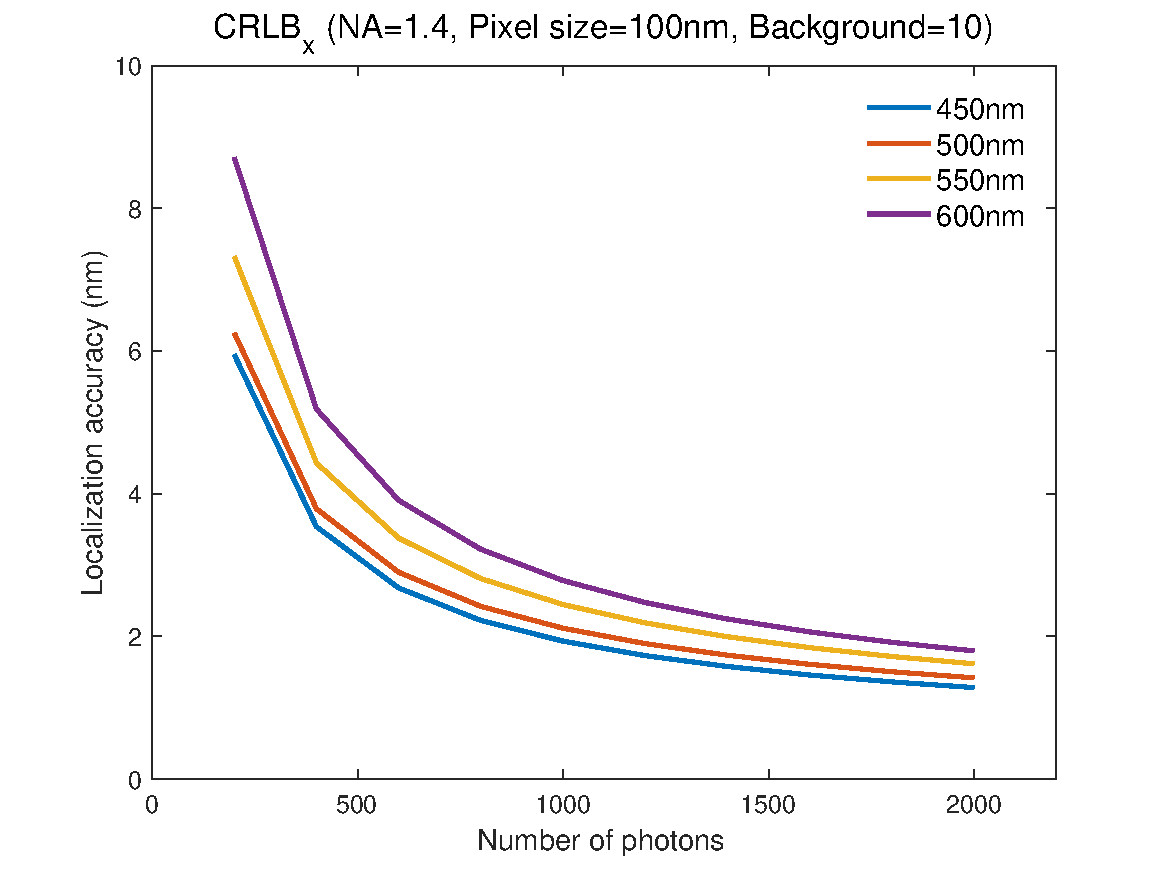
\includegraphics[width=0.5\textwidth]{SaveFilex} &
        %\column{.5\textwidth}
        %\centering
        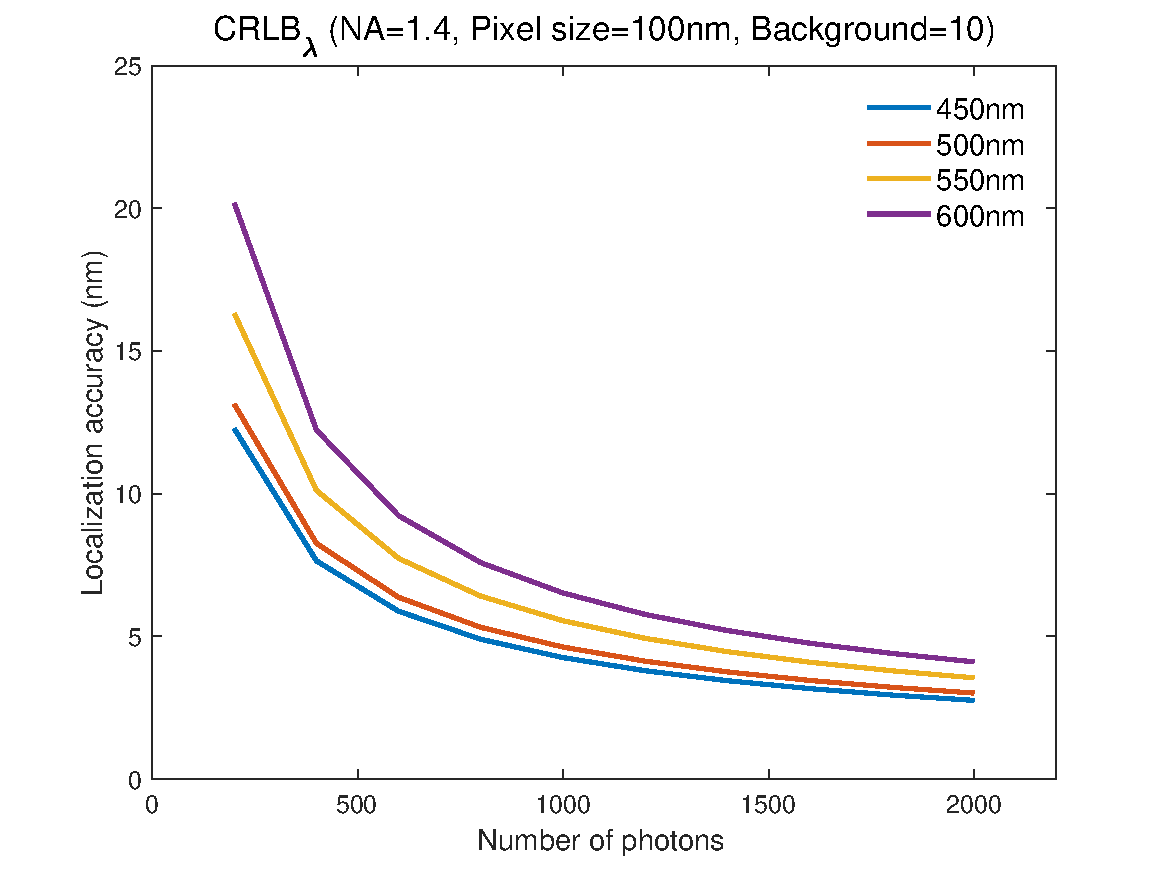
\includegraphics[width=0.5\textwidth]{SaveFilel} \\
    \end{tabular}
\end{frame}

\begin{frame}{
    Impact of Defocusing 
}
    \begin{itemize}
        \item Defocusing introduces biasing to wavelength estimation 
    \begin{itemize}
        \item Accuracy bound should take into account both bias \& CRLB
    \end{itemize}
        \item Generalized CRLB in presence of bias
            \begin{gather*}
                \textrm{Var}(\hat{\lambda})\geq\frac{\left[1+b'(\lambda)\right]^2}{I(\lambda)}\\
                b(\lambda)\text{: bias},\: I(\lambda)\text{: Fisher information}
            \end{gather*}
        \item CRLB is z dependent
            \begin{gather*}
                b(\lambda) = \lambda(M(z)-1),\quad b'(\lambda) = M(z)-1\\
                \textrm{Var}(\hat{\lambda})|_{z}\geq\frac{M(z)^2}{I(\lambda)|_{z}}\\
                M(z)\textsf{: magnification factor of the PSF at $z$}
            \end{gather*}
    \end{itemize}
\end{frame}

\begin{frame}{
    Impact of Defocusing 
}
    \begin{itemize}
        \item Assuming certain distribution for $z$, performance bound in presence of $z$ variation can be calculated  
    \begin{itemize}
        \item Mean squared error at $z$: $E[(\hat{\lambda}-\lambda)^2]|_z = \textrm{Var}(\hat{\lambda})|_{z} + b(z)^2 $
        \item Final CRLB is calculated as a weighted sum over $z$
\begin{align*}
    CRLB_{\lambda} &= \int_{z_{min}}^{z_{max}} E[(\hat{\lambda}-\lambda)^2] f(z)dz \\
                   &= \int_{z_{min}}^{z_{max}}{\left(\textrm{Var}(\hat{\lambda})|_{z}+b(\lambda)^2\right)f(z)dz}\\
                   &\geq 2\int_{0}^{\Delta z_{max}}{\left(\frac{M(z)^2}{I(\lambda)|_z}+\lambda^2 (M(z)-1)^2\right)f(z)dz}
\end{align*}
    \item PSF Symmetry over $z$, $f(z)$: probability distribution of $z$
        \item For $M(z)=1$, converges to the CRLB at $z=0$
    \end{itemize}
    \end{itemize}
\end{frame}

\begin{frame}{
    Impact of Defocusing 
}
    \begin{itemize}
        \item   Magnification factor \& Fisher information vs. $z$
    \begin{itemize}
        \item    $N_{photon}$=1500, $\lambda$=600nm, $n_i$=1.5, Born \& Wolf model
    \end{itemize}
    \end{itemize}
    \vspace{-1em}
    \centering
    \begin{tabular}{C{0.45\textwidth} C{0.45\textwidth}}
        %\column{.5\textwidth}
        %\centering
        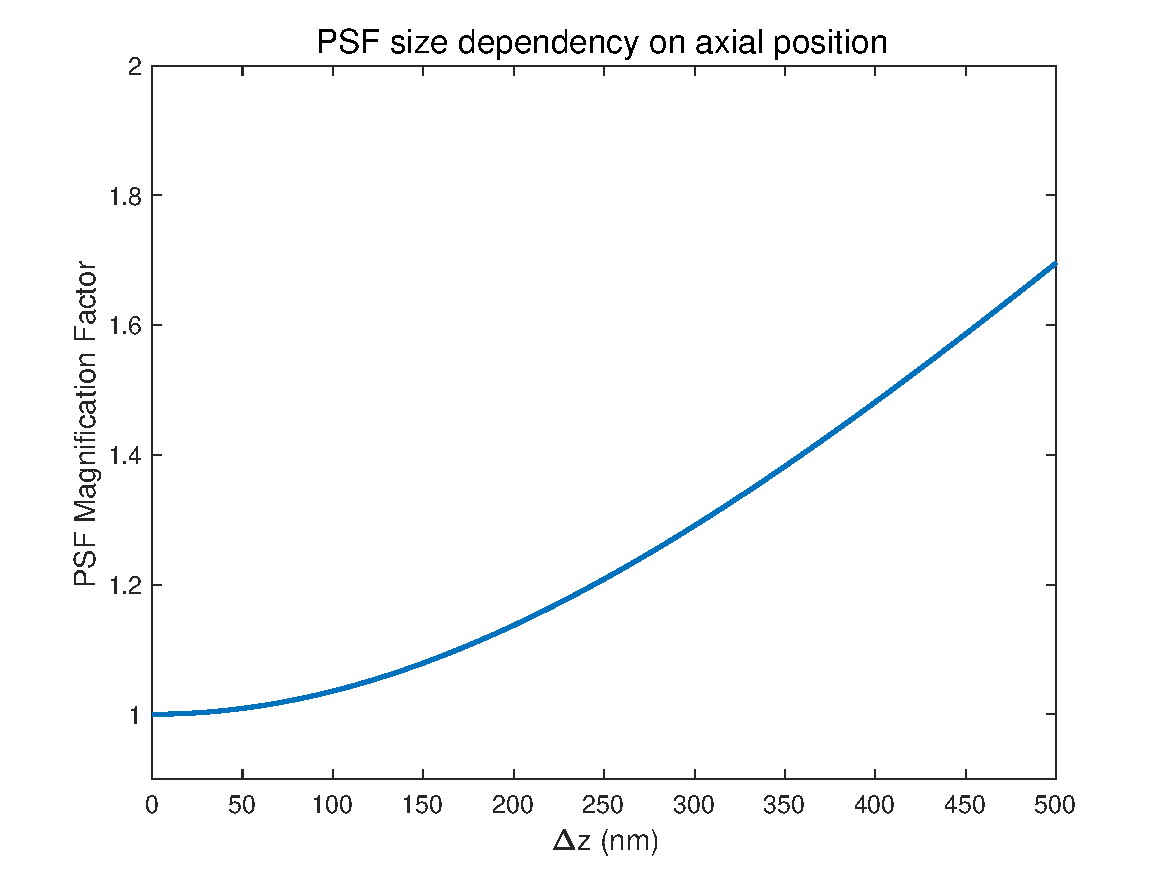
\includegraphics[width=0.5\textwidth]{SaveFilemag} &
        %\column{.5\textwidth}
        %\centering
        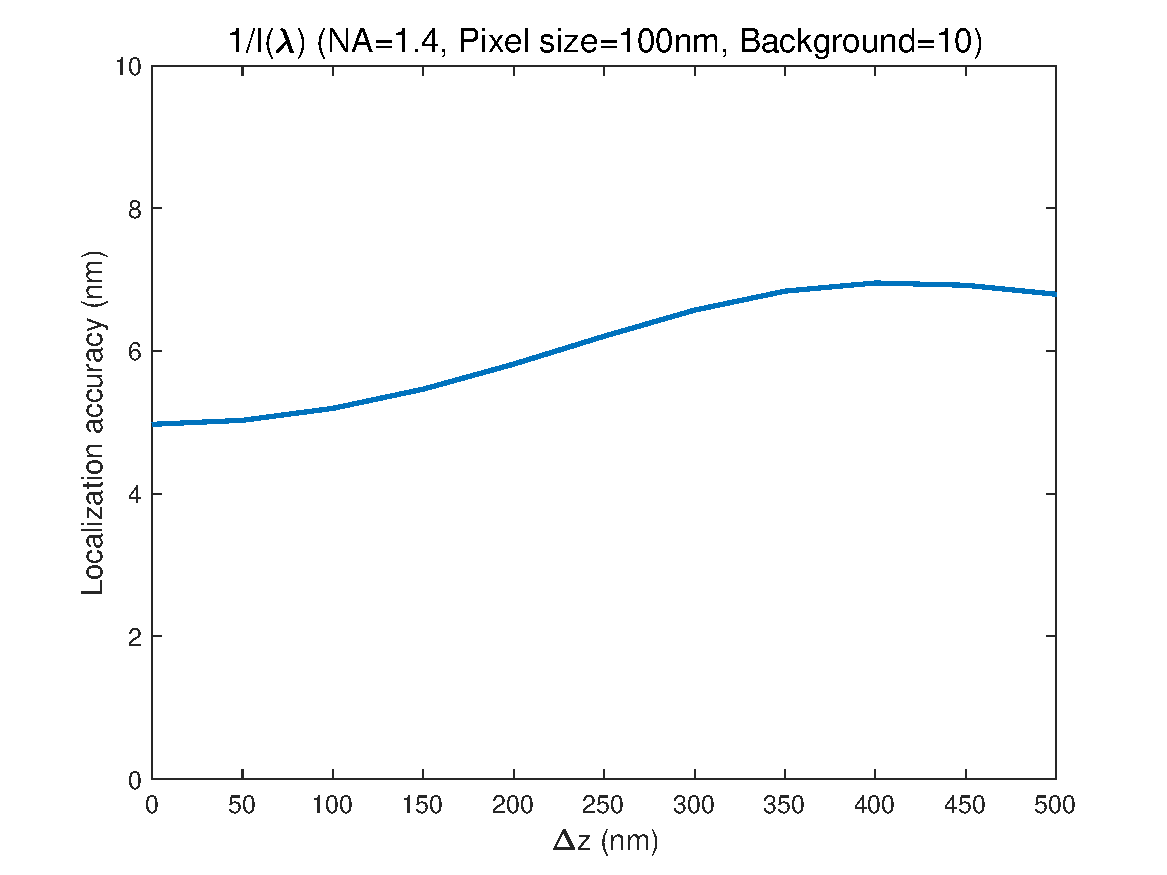
\includegraphics[width=0.5\textwidth]{SaveFilez} \\
    \end{tabular}
    \begin{itemize}
        \item For $\Delta z_{max}$=100nm \& $f(z)$=uniform, CRLB=9.86nm \\(originally 4.97nm)
        \item For $\Delta z_{max}$=500nm, CRLB=177nm!
    \end{itemize}
\end{frame}

\begin{frame}{
    3D+Color: Multifocal Plane
    }
    \vspace{-1em}
    \begin{tabular}{C{0.45\textwidth} C{0.45\textwidth}}
    \begin{itemize}
        \item Total Fisher information matrix is the sum of FI from each imaging plane \footlessfullcite{biplane}
            \begin{gather*}
                I_{tot}(\boldsymbol{\theta}) = \sum_{i=1}^{N_{plane}}{I_{i}(\boldsymbol{\theta})}
            \end{gather*}
        \item Biplane setting
    \begin{itemize}
        \item    $N_{photon}$=1500, $\lambda$=600nm
        \item 50/50 beam split \\(750 photons/plane)
        \item Distance between planes: 500nm
    \end{itemize}
    \end{itemize}
    & 
            \centering
            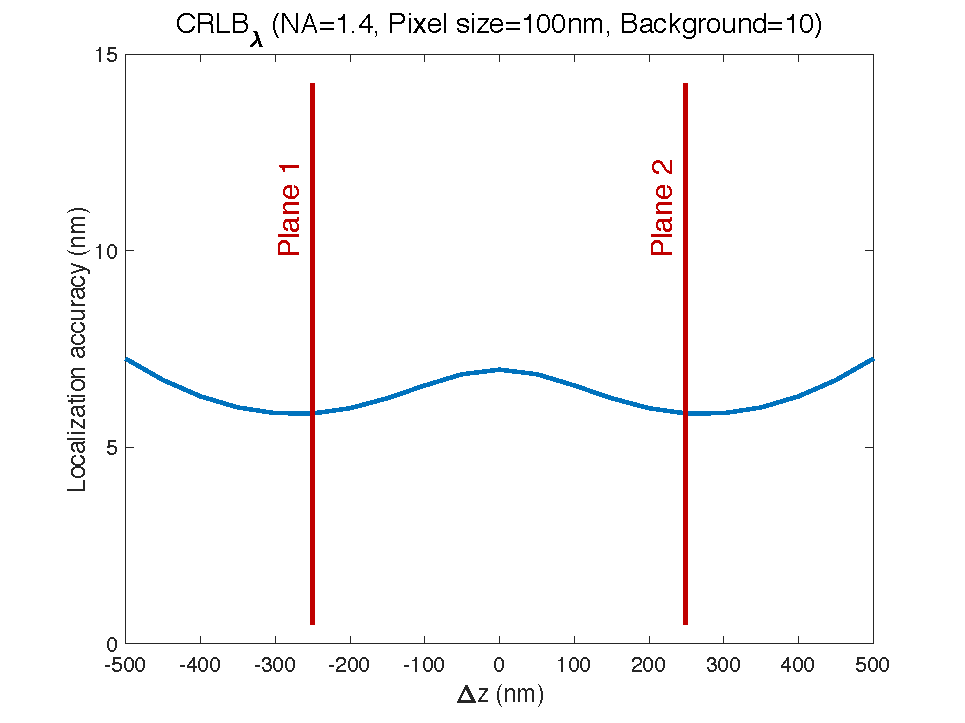
\includegraphics[width=0.5\textwidth]{bp}
            \\
        \end{tabular}
    %\vfill
    %\begin{center}
        %You can also draw figures in \LaTeX{} using the PSTricks package.
    %\end{center}
\end{frame}

\begin{frame}{
        3D+Color: Double Helix/Astigmatic\footlessfullcite{delft} 
    }
    \includegraphics<1>[width=\textwidth]{dh1}
    \includegraphics<2>[width=\textwidth]{dh2}
    %\vfill
    %\begin{center}
        %You can also draw figures in \LaTeX{} using the PSTricks package.
    %\end{center}
\end{frame}

\begin{frame}{
    Conclusions
}
    \begin{itemize}
        \item Takeaways from CRLB calculation
    \begin{itemize}
        \item Can work with useful accuracy ($\sim$10nm) only when $z$ \& $\lambda$ are disentangled
        \item Looks promising for biplane \& dual helix PSF
    \end{itemize}
        \item Next steps:
    \begin{itemize}
        \item Fluorophore spectrum/dipole moment dependence 
    \begin{itemize}
        \item If there's a performance difference between beads and single molecule, this could be the reason 
    \end{itemize}
            \vspace{0.1em}
        \item Quantitative comparison with chromatic dispersion-based methods
            \vspace{0.1em}
        \item Characterize readout noise
            \vspace{0.1em}
        \item Actual PSF \& chromatic aberration analysis for microscopes in the lab 
        \begin{itemize}
            \item Tools such as PSFj\footlessfullcite{psfj} can be applied
            \vspace{0.1em}
        \end{itemize}
        \item Compare to the fitted simulation dataset or experimental data
            \vspace{0.1em}
        \item Right fitting algorithm to achieve close-CRLB performance
    \end{itemize}
    \end{itemize}
\end{frame}

%\begin{frame}{Chirp Loop}
%    \centering
%        \resizebox{0.9\textwidth}{!}{
%    % Title: Block diagram of Third order noise shaper in Compact Disc Players
% Author: Ramón Jaramillo
%\documentclass[tikz,14pt,border=10pt]{standalone}

%\begin{document}
% Definition of blocks:
\tikzset{%
	block/.style    = {fill=white, draw, thick, rectangle, minimum height = 3em, minimum width = 3em},
  	sum/.style      = {fill=white, draw, circle, minimum size=0.7cm, node distance = 2cm}, % Adder
	point/.style 	= {
		circle,inner sep=0pt,minimum size=0pt,fill=black,draw=black
	},
	cross/.style = {
		cross out, 
		draw=black, 
		minimum size=2*(#1-\pgflinewidth), 
		inner sep=0pt, 
		outer sep=0pt
	},
	cross/.default = {
		1pt
	},
  	input/.style    = {coordinate}, % Input
  	output/.style   = {coordinate} % Output
}
% Defining string as labels of certain blocks.

\definecolor{myblue}{RGB}{75,213,217}
\definecolor{mygreen}{RGB}{189,242,113}

\newcommand{\suma}{\Large$+$}
\newcommand{\lo}{\Large$\sim$}
\newcommand{\inte}{{$\bigintssss$}}
\newcommand{\derv}{\Large$\tau\frac{d}{dt}$}
\newcommand*{\myfont}{\fontfamily{phv}\selectfont}
\newcommand*{\mfm}[1]{ { \textrm{\myfont{\textit{{#1}}}} } }

\begin{tikzpicture}[auto, thick, node distance=2cm, >=triangle 45]
\draw
    % Drawing the blocks of first filter :
    %node at (0,0)[right=-3mm]{\Large \textopenbullet}
    %node [input, name=input1, point, circle, draw, fill=white, minimum size=3pt] {} 
	node [sum, name=input1, label={below:\myfont{LO}}] {} node at (input1) [yshift=-0.5mm] {\lo} 
	%node [sum, right of=input1] (suma1) {} node at (suma1) [cross=5pt, very thick, rotate=45] {} 
	node [block, right of=input1] (pfd) {\myfont{PFD}}

	node [point, right of=pfd, minimum size=4pt, xshift=-0.5cm] (pt1) {}
	node [sum, right of=pt1, xshift=-0.5cm, yshift=1cm] (prop) {} node at (prop) [cross=5pt, thick] {}
	node [sum, right of=pt1, xshift=-0.5cm, yshift=-1cm] (intp) {} node at (intp) [cross=5pt, thick] {}
	node [above of=prop, yshift=-0.7cm] (alpha) {$\alpha$}
	node [below of=intp, yshift=0.7cm] (beta) {$\beta$}
	node [block, right of=intp] (acc) {\Large$\Sigma$}
	node [sum, right of=acc, xshift=-0.5cm, yshift=1cm] (sum) {} node at (sum) [cross=5pt, thick, rotate=45] {}


    node [block, right of=sum] (inte) {\inte}
	%node [point, right of=inte,xshift=-0.5cm, minimum size=1pt] (pt1) {}

	node [block, right of=inte, xshift=0.5cm] (laser) {\myfont{Laser}}

	node [block, below of=laser, yshift=-1cm, label={below:\myfont{MZI+PD}}] (diff) {\derv};
    % Joining blocks. 
    % Commands \draw with options like [->] must be written individually
	\draw (pfd) -- (pt1.center);

    \draw[->](input1) -- node {}(pfd);
    \draw[->](sum) -- node {} (inte);
    \draw[->](pt1.center) |- node {} (prop);
    \draw[->](pt1.center) |- node {} (intp);
    \draw[->](intp) -- node {} (acc);
    \draw[->](prop) -| node {} (sum);

    \draw[->](alpha) -- node {} (prop);
    \draw[->](beta) -- node {} (intp);

    \draw[->](acc) -| node {} (sum);
    \draw[->](inte) -- node {} (laser);
    \draw[->](laser) -- node {} (diff);
    \draw[->](diff) -| node[near end]{} (pfd);
    % Adder
%\draw
    %node at (5.4,-4) [sum, name=suma2] {\suma}
        %% Second stage of filter 
    %node at  (1,-6) [sum, name=suma3] {\suma}
    %node [block, right of=suma3] (inte2) {\inte}
    %node [sum, right of=inte2] (suma4) {\suma}
    %node [block, right of=suma4] (inte3) {\inte}
    %node [block, right of=inte3] (Q2) {\Large$Q_2$}
    %node at (9,-8) [block, name=ret2] {\Large$T_2$}
%;
    %% Joining the blocks of second filter
    %\draw[->] (suma3) -- node {} (inte2);
    %\draw[->] (inte2) -- node {} (suma4);
    %\draw[->] (suma4) -- node {} (inte3);
    %\draw[->] (inte3) -- node {} (Q2);
    %\draw[->] (ret2) -| (suma3);
    %\draw[->] (ret2) -| (suma4);
         % Third stage of filter:
    % Defining nodes:
%\draw
    %node at (11.5, 0) [sum, name=suma5]{\suma}
    %node [output, right of=suma5]{}
    %node [block, below of=suma5] (deriv1){\derv}
    %node [output, right of=suma5] (sal2){}
%;
    %% Joining the blocks:
    %\draw[->] (suma2) -| node {}(suma3);
    %\draw[->] (Q1) -- (8,0) |- node {}(ret1);
    %\draw[->] (8,0) |- (suma2);
    %\draw[->] (5.4,0) -- (suma2);
    %\draw[->] (Q1) -- node {}(suma5);
    %\draw[->] (deriv1) -- node {}(suma5);
    %\draw[->] (Q2) -| node {}(deriv1);
        %\draw[<->] (ret2) -| node {}(deriv1);
        %\draw[->] (suma5) -- node {$Y(Z)$}(sal2);
        %% Drawing nodes with \textbullet
%\draw
	%node [point, circle, minimum size=3pt] at (8,0) {} 
	%node [point, circle, minimum size=3pt] at (8,-2) {} 
	%node [point, circle, minimum size=3pt] at (5.4,0) {} 
	%node [point, circle, minimum size=3pt] at (5,-8) {} 
	%node [point, circle, minimum size=3pt] at (11.5,-6) {} 
	%node at (8,-2){\textbullet}
	%node at (5.4,0){\textbullet}
		%node at (5,-8){\textbullet}
		%node at (11.5,-6){\textbullet}
		%;
	% Boxing and labelling noise shapers

	\begin{pgfonlayer}{background}
		%\fill [rounded corners,fill=mygreen,thick](-0.8,-3.25) rectangle (7,1);
		%\fill [rounded corners,fill=myblue,thick](7.25,-3.25) rectangle (9.5,1);
	\end{pgfonlayer}
	\draw [dashed, thick] ($(pfd.east)+(0.5,-2.6)$) rectangle ($(sum.center)+(0.6, 2.6)$);
	%\node at() {LF}; 

	%\node at (-0.5,1) [above=5mm, right=0mm] {\textsc{first-order noise shaper}};
	%\draw [color=gray,thick](-0.5,-9) rectangle (12.5,-5);
	%\node at (-0.5,-9) [below=5mm, right=0mm] {\textsc{second-order noise shaper}};

\end{tikzpicture}

%\end{document}

%}
%\end{frame}


%\begin{frame}{An Overview of \LaTeX{}}
%    \begin{enumerate}
%    	\item What \LaTeX{} is and how to get it
%        \item Making documents
%        \item Making presentations using \texttt{Beamer}
%        \item Making posters using \texttt{Beamerposter}
%        \item Rapid document/presentation prep (Markdown + \LaTeX{})
%     \end{enumerate}
%     \vfill
%     A \LaTeX{} cheat sheet is available here:      \url{http://www.stdout.org/~winston/latex/latexsheet.pdf}
%\end{frame}

%\begin{frame}{\LaTeX{} is a typesetting language.}

%    \begin{itemize} % You can also use   (\setbeamercovered{transparent=30}) to set transparency
%  	\item It lets you \textcolor{red}{seamlessly} transition between words and math: 
%  	$$\sum_{n=0}^\infty\frac{x^n}{n!}=e^x$$
%  	\item You can typeset \textcolor{red}{publish-quality} articles, books, theses, presentations, and posters
%  	\item It \textcolor{red}{automatically} handles bibliography, equation, image, and table references
%  	\item The easy part is learning how to type math, the hard part is the formatting
%  		\begin{itemize}
%    		\item But luckily, there is a \textbf{huge} user-base with lots of examples
%    	\end{itemize}
%    \end{itemize}
    
%\end{frame}
    
%\begin{frame}{\LaTeX{} can be used at home or online.}

%    \begin{itemize}
%    	\item You can download \LaTeX{} distributions and editors here: \url{http://latex-project.org/ftp.html}
%        \item There are also online compilers/editors
%        \begin{itemize}
%        	\item \url{http://writelatex.com}
%        	\item \url{http://sharelatex.com}
%        \end{itemize}
%        \item There are also ways to write in Markdown that recognize \LaTeX{} syntax (great for notes, research, quick presentations)
%         \begin{itemize}
%        	\item \url{http://stackedit.io}
%        	\item IPython
%        \end{itemize}
%    \end{itemize}
%\end{frame}

%\begin{frame}[fragile]{Hello World.}
%            \begin{verbatim}
%           	\documentclass[10pt]{article}
%           	 ...
%           	\begin{document}
%           	 Hello World.
%            \end{document}
%    		\end{verbatim}
% 	\vfill

%    	Curly braces are a staple of \LaTeX{}. They're used for arguments, setting environments, and telling \LaTeX{} what belongs where. For example, $\sum_{n=0}$ is written \verb!\sum_{n=0}! instead of \verb!\sum_n=0!, which gives $\sum_n=0$. Square braces are for options (paper size, font size, etc.). 

%\end{frame}

%\begin{frame}[fragile]{Hello World.}
%            \begin{verbatim}
%           	\documentclass[10pt]{article}
%           	 ...
%           	\begin{document}
%           	 Hello World.
%            \end{document}
%    		\end{verbatim}
% 	\vfill

%    \begin{block}{Important}

%    	Curly braces are a staple of \LaTeX{}. They're used for arguments, setting environments, and telling \LaTeX{} what belongs where. For example, $\sum_{n=0}$ is written \verb!\sum_{n=0}! instead of \verb!\sum_n=0!, which gives $\sum_n=0$. Square braces are for options (paper size, font size, etc.). 

%    \end{block}
%\end{frame}

%\begin{frame}[fragile]{Making Documents}

%    \begin{itemize}
%    	\item Inserting figures (\verb!graphicx! package)
%        \item Making tables (\verb!tabular! and \verb!table! environment)   
%        \item Typesetting math (\verb!$!, \verb!$$!, \verb!equation!, \verb!align!)
%    \end{itemize}

%\end{frame}

%\begin{frame}[fragile]{Making presentations with Beamer.}

%    The structure goes something like this:
%    \begin{verbatim}
%    \documentclass{beamer}
%    \mode<presentation>
%    \usetheme{default}
%    ...other theme options (insert watermark, etc.)
    
%   \begin{document}
    
%    	\begin{frame}
%    		...
%    	\end{frame}
        
%    \end{document}
%    \end{verbatim}
%    \vfill
%    You can insert transitions, animations, slow reveals, etc.
%\end{frame}

%\begin{frame}{Here's a Beamer example.}
%    \begin{columns}
%    	\column{0.5\textwidth}
%        	\begin{itemize}
%            \item<1-> Here's my first point 
%            \item<2-> And my second 
%            \item<3-> And my third
%            \end{itemize}
%        \column{0.5\textwidth}
%            \centering
%            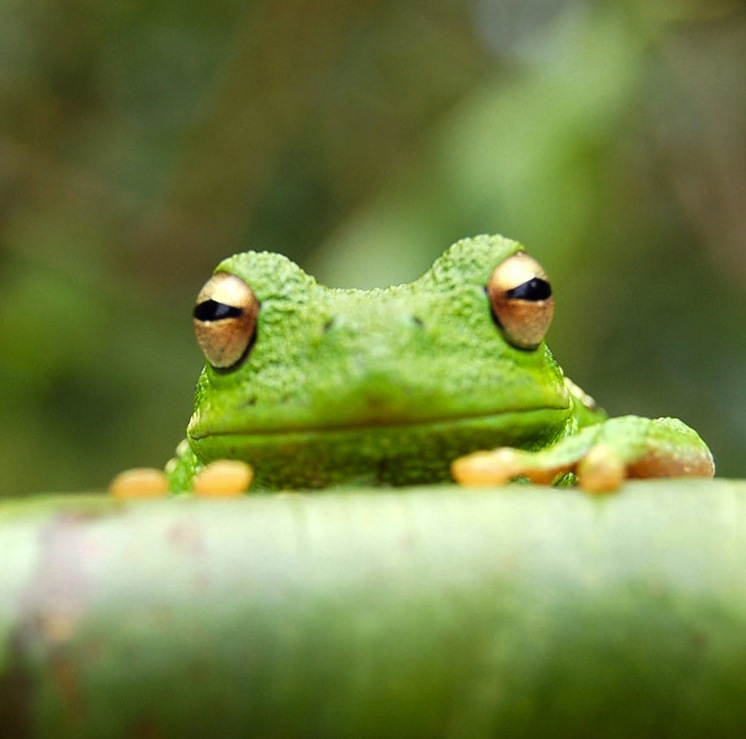
\includegraphics[width=2in]{frog.jpg}
%    \end{columns}
%    \vfill
%    \begin{center}
%    	You can also draw figures in \LaTeX{} using the PSTricks package.
%    \end{center}
%\end{frame}

%\begin{frame}{Making a poster using the beamerposter package.}
%    \begin{itemize}
%    	\item All commands are essentially the same to the \texttt{beamer} package
%    	\item Still working on the style file
%        \item Sections are broken out using the \texttt{block} command
%    \end{itemize}
%\end{frame}


%\begin{frame}[fragile]{BibTeX handles making the references and making the bibliography.}
%    \begin{columns}
%    	\column{0.5\textwidth}
%        	\begin{itemize}
%            \item Just put your references (automatically generated by Google Scholar) in a .bib file that you reference at the end of the document, 
%            \item JabRef is also a powerful citation manager: \url{http://jabref.sourceforge.net/}
%            \item You can also change the citation style: [Number], (Author,Year), etc. 
%            \end{itemize}
%        \column{0.5\textwidth}
%            \centering
%            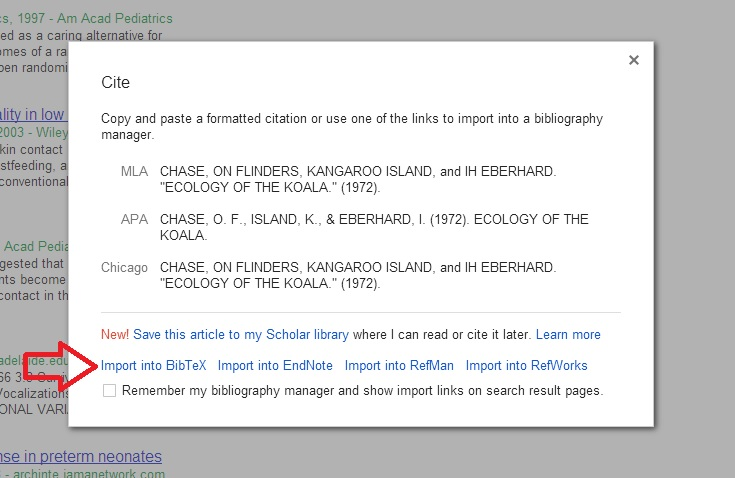
\includegraphics[width=2in]{ScholarPic.jpg}
%    \end{columns}
%    \vfill
%    Just include \verb!\bibliographystyle{plain}! in the preamble and 	\verb!\bibliography{yourrefname.bib}! before the end of the doc.
%\end{frame}

%\begin{frame}{Quick prep: Markdown + \LaTeX{}}

%    \begin{itemize}
%    \item You can avoid formatting the documents and just get to the sweet, sweet math
%    \item iPython and \url{stackedit.io} both have Markdown environments that can render \LaTeX{} using MathJax, a Javascript tool
%    \item You can make quick presentations (in IPython), notes, handouts, etc.
    
%    \end{itemize}

%\end{frame}
%\printbibliography


\end{document}
